% PROGETTAZIONE 
\chapter{Progettazione}\label{chap:design}

\section {Progettazione architetturale}
\subsection{Architettura OpenChat}
Avendo dovuto basare l'applicazione sulla soluzione già implementata per il web dalla zimlet OpenChat è utile approfondire la sua architettura per comprendere le differenze applicate. \\
La comunicazione tra il server Zimbra e la zimlet OpenChat avviene attraverso una struttura SOAP, protocollo per lo scambio di messaggi tra componenti hardware.
Questa struttura, nel caso della zimlet OpenChat, permette la comunicazione con il server indirettamente facendo passare gli eventi per il web client Zimbra che li gestisce in base ai propri bisogni prima di inviarli al server. \\
\begin{figure}[H] 
	\centering
	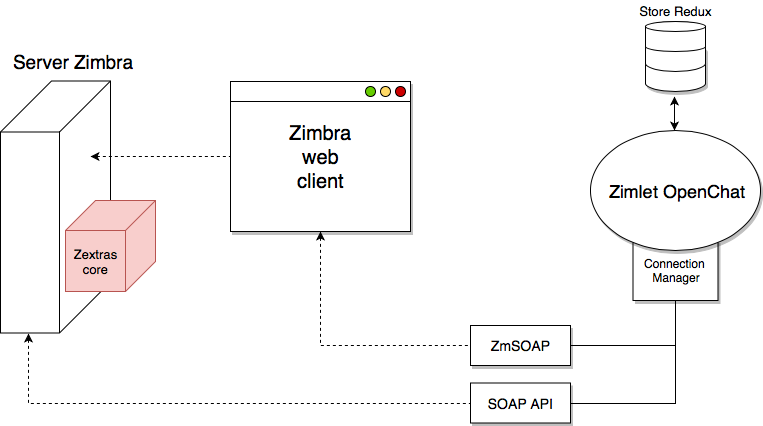
\includegraphics[scale=0.45]{architettura2}
	\caption{Architettura OpenChat}
\end{figure}
Dato che l'applicazione Teamwork non interagisce con Zimbra web client è stata modificata la modalità di ricezione ed invio dei messaggi SOAP e la gestione tramite connection manager in modo da far comunicare direttamente Teamwork e il server Zimbra (con Zextras core integrato).

\subsection{Gestione eventi}
Per gestire in modo ottimale ed efficacie la comunicazione tra server e client è stata strutturata un'architettura capace di reagire alla ricezione e all'invio di eventi. \\
Questa struttura permette la sincronizzazione dei dati tra il server e tutte le sessioni aperte facendo in modo di tenere aggiornato lo store Redux di ogni applicazione connessa.\\
Di seguito un'approfondimento delle varie componenti che permettono questa interazione:
\begin{figure}[H] 
	\centering
	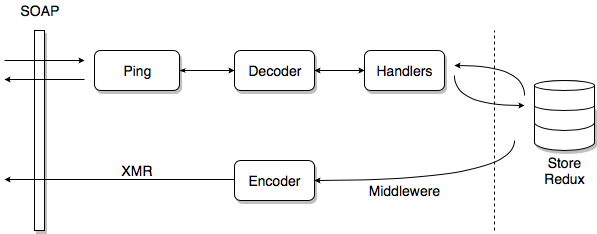
\includegraphics[scale=0.6]{architettura}
	\caption{Gestione eventi}
\end{figure}
\subsubsection{SOAP}
La trasmissione e la negoziazione dei messaggi scambiati tra server e client è regolata secondo i protocolli HTTP o SMTP, all'interno dei quali viene incapsulato il messaggio SOAP.
I messaggi SOAP, rappresentati in figura \ref{fig:SOAP}, sono basati sul metalinguaggio XML e vengono strutturati secondo due segmenti principali, head e body. 
\begin{figure}[H] 
	\centering
	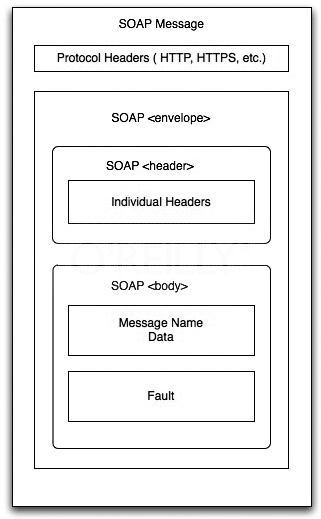
\includegraphics[scale=0.4]{SOAP}
	\caption{Struttura messaggio SOAP}
	\label{fig:SOAP}
\end{figure}
\begin{itemize}
	\item Il segmento Header contiene metadati utili per la trasmissione del messaggio, come informazioni per il routing e per la sicurezza. Può essere opzionale.
	\item Il segmento Body, che invece risulta obbligatorio, trasporta il contenuto informativo (payload) del messaggio. Saranno questi i dati importanti per la gestione delle informazioni.
\end{itemize}
Per ogni SOAP request inviata al server ci sarà una SOAP respose in ritorno. Questa risposta può contenere dati richiesti dalla precedente SOAP request, informazioni sullo stato del server o possibili errori di risposta.
\subsubsection{Connection Manager}
È il Connection Manager ad occuparsi degli eventi in arrivo dal server. Per fare ciò ha bisogno di due componenti principali:
\begin{itemize}
	\item il Ping, componente che si occupa di stabilire una connessione con il server e di mantenerla operativa durante tutta la sessione. In questo modo l'applicazione rimarrà sempre in ascolto di nuovi eventi provenienti dal server;
	\item il Decoder, componente che, una volta ricevuto un messaggio SOAP dal Ping, ne decodificherà il body permettendo una più facile comprensione del contenuto. Si è utilizzato un Abstract Factory per la creazione di questa componente, design pattern che fornisce un’interfaccia per creare famiglie di prodotti senza specificare classi concrete.
\end{itemize}
\subsubsection{Handlers}
Questa famiglia di componenti riceve in input degli eventi provenienti dal Decoder. Questo vuol dire che non riceve dei generici messaggi SOAP ma dei JSON associati a dei particolari eventi di cui è stato implementato un handler specifico.\\
La sua funzione, quindi, è quella di modificare lo stato dello store Redux, basandosi sui dati ricevuti, attraverso un dispatcher che modifica il flusso dei dati utilizzati nell'applicazione in modo unidirezionale, così da non creare inconsistenza.
\subsubsection{Encoder}
Gli eventi possono essere generati anche dall'applicazione e per gestire il bisogno di propagare le modifiche che vengono fatte allo store Redux al server (con la successiva propagazione dei dati verso le altre sessioni) è stato introdotto un encoder, il corrispondente del precedente componente decoder per l'invio degli eventi. \\
Quando viene fatto il dispatch di un'azione con la conseguente modifica dello store vengono invocati dei particolari middleware che si occupano dell'invio dell'evento all'encoder corrispondente. Questa componente permette la traduzione dell'evento in un messaggio SOAP generico comprensibile dal server.
\section{Progettazione grafica}
Prima di procedere alla definizione delle classi necessarie per l'implementazione 
dell'applicazione è stato deciso di effettuare la progettazione della UI per far 
si che il progetto di stage abbracciasse a 360 gradi il processo di sviluppo di 
un'applicazione da parte di un'azienda.

\subsection{Wireframe}
In base ai requisiti e agli use case raccolti è stato definito il modello iniziale
 dell'applicazione tramite la realizzazione dei wireframe delle varie schermate. \\
Questo studio è la prima rappresentazione visuale dell'applicazione ed ha lo 
scopo di identificare la struttura, l'architettura dell'informazione e la 
disposizione degli elementi nella pagina.\\
Di seguito vengono riportati i wireframe sviluppati di alcune delle pagine più 
importanti di Teamwork:
\begin{figure}[H] 
	\centering
	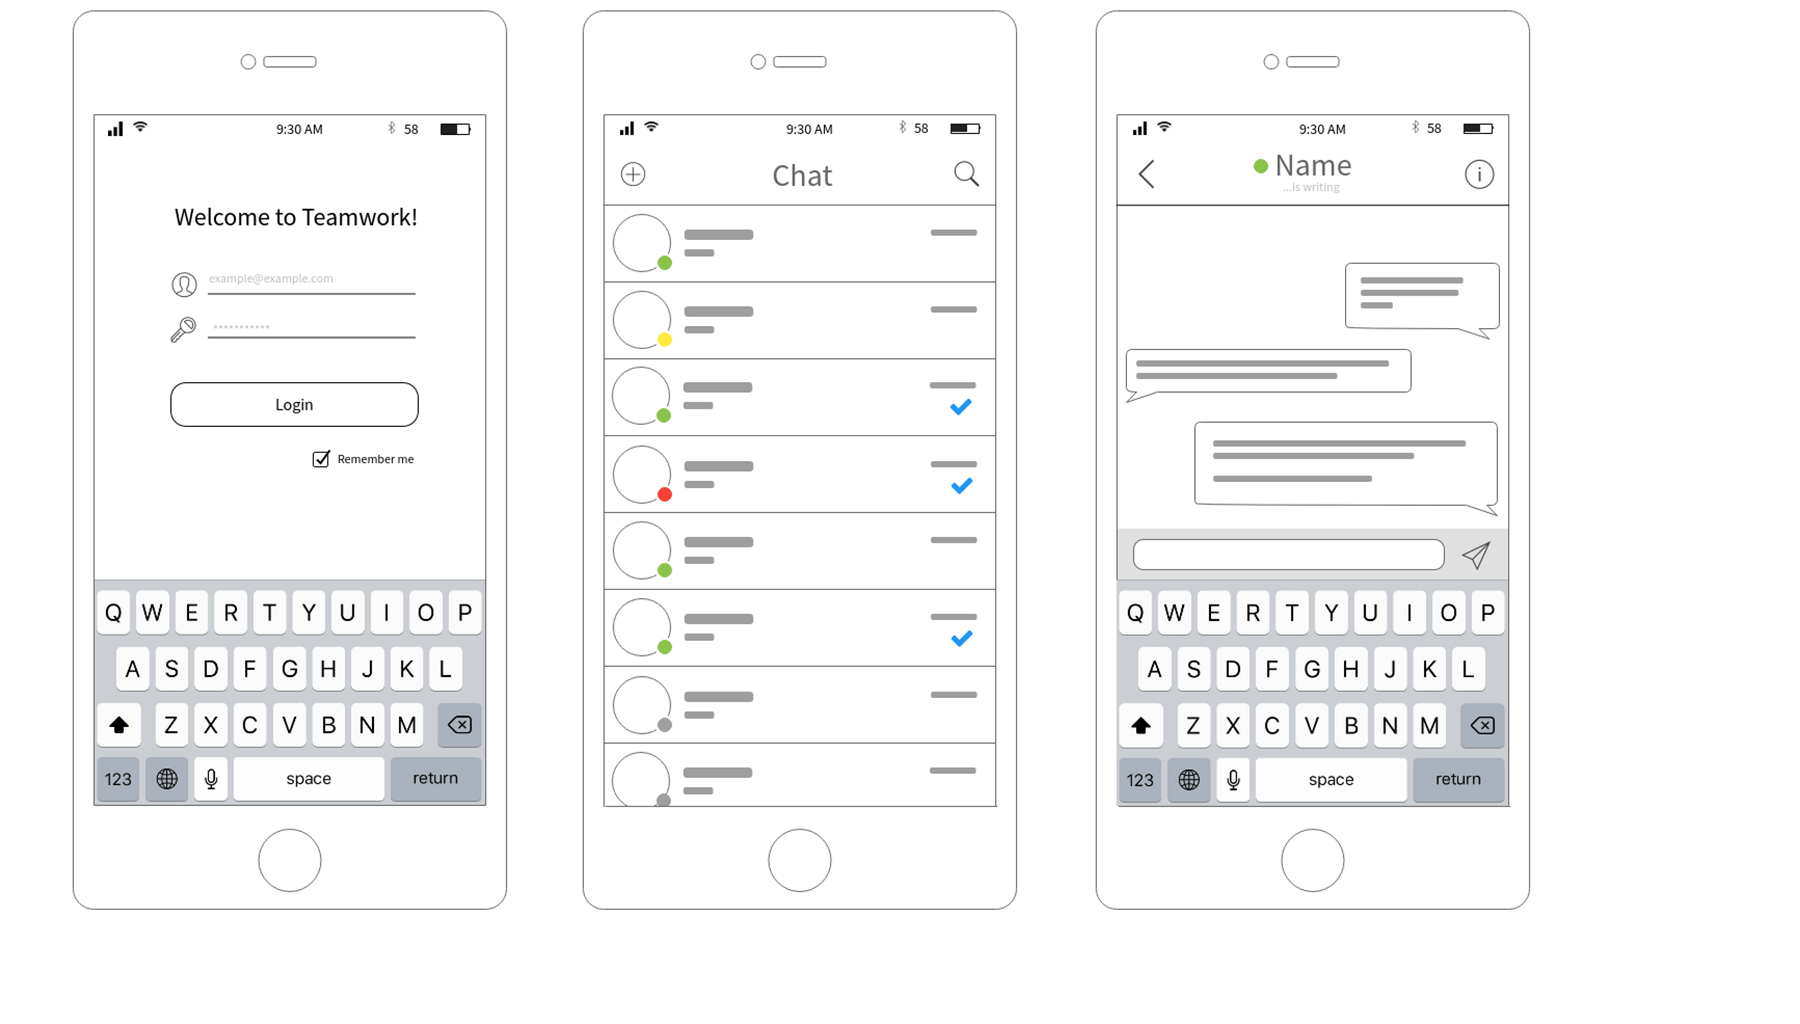
\includegraphics[scale=0.5]{wireframe}
	\caption{Wireframe pagina di login, buddylist e chat page.}
\end{figure}
Come possiamo notare dagli esempi riportati, in questa fase non è stato deciso 
nulla riguardo la rappresentazione grafica dei vari elementi. 
Si è definita soltanto la struttura delle varie schermate, il collegamento tra 
di esse e quali elementi realmente soddisfino i requisiti già studiati. 
Il risultato, comunque, è stato molto vicino alla GUI ottenuta alla fine della 
codifica in quando i wireframe sono stati disegnati tenendo conto della 
soluzione web già presente.\\ 
Questo passo è stato essenziale per rendere più chiara l'idea del prodotto desiderato.

\subsection{Linee guida}
Per quanto riguarda la GUI vera e propria sono state fornite dall'azienda delle 
guidelines da seguire per la rappresentazione grafica di ogni elemento. \\
Nello specifico le guidelines toccano temi come:
\begin{itemize}
	\item le proporzioni tra i componenti;
	\item i colori da utilizzare;
	\item le definizioni di alcuni elementi base;
\end{itemize}
Questo serve per avere uno stile comune tra le varie applicazioni che 
l'azienda sviluppa. \\
Un esempio è la definizione del componente "card", destinato alla 
visualizzazione dei dettagli relativi ad un buddy:
\begin{figure}[H] 
	\centering
	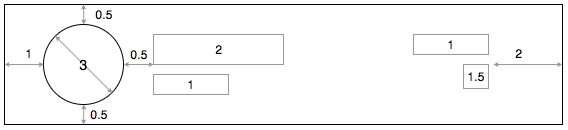
\includegraphics[scale=0.5]{guidelines}
	\caption{Esempio guidelines spazi}
\end{figure}
Si noti come ogni elemento sia posizionato in modo preciso definendo delle 
proporzioni tra gli spazi. In questo modo la successiva codifica dello stile sarà 
assolutamente definita da regole precise in modo da non dover interagire in modo 
continuativo con il responsabile grafico del progetto. \\
L'applicazione delle guidelines nel codice è avvenuta in parallelo con lo sviluppo 
in quando, seguendo una metodologia agile, si è ritenuto opportuno che le varie 
versioni prototipali dell'applicazione avessero anche una progressiva applicazione 
delle regole di stile.\\
Approvati i wireframe è stato possibile proseguire alla definizione di tutti 
e soli i componenti veramente utili al layout.

\section{Progettazione di dettaglio}
